\section{Introduction}


As digital images began to be stored and transmitted over networks, the need to reduce their size became essential.
In natural photographic images, neighboring pixels tend to be highly correlated; for example,
a pixel in a sky region usually has color values similar to its surrounding pixels.
Compression algorithms exploit this spatial redundancy to efficiently reduce image data without significant loss of quality.
Codecs start the compression scheme by transforming input image into an intermediate representation, that has better statistical parameters for
entropy encoding. Historically most popular such transformations were DCT (Discrete Cosine Transform) and DWT
(Discrete Wavelet Transform), both of which transform the input space by dividing it into a grid of blocks and then
performing further operations within each one. Such transformed image still contains a lot of information that is missed
by human vision. Alterations in high-frequency components are generally less perceptible to the visual cortex. To further diminish the size of the transformed representation, quantization is employed in lossy codecs to effectively discard those values that remain undetected.
This approach proved to achieve best results in modern codecs, but with harsher
quantization in lossy compression block boundaries are much more visible. 
Lossless codecs often used block lattices for context modelling and better prediction of residuals. Each block is directly adjacent 
to 4 different blocks and can infer its values from those neighbors. In JPEG-LS \cite{weinberger1996LOCO} authors proposed a predictor
LOCO-I that assigns each element to one of 365 contexts based on the already decoded neighboring values adjusting 
the distributions of encoded elements. Such grouping enables codec to use different instances of entropy coder for 
different probability distributions observed within each context.

\begin{figure}[ht]
    \centering
    {
    \setlength{\fboxsep}{0pt}
    \setlength{\fboxrule}{1pt}
    \fbox{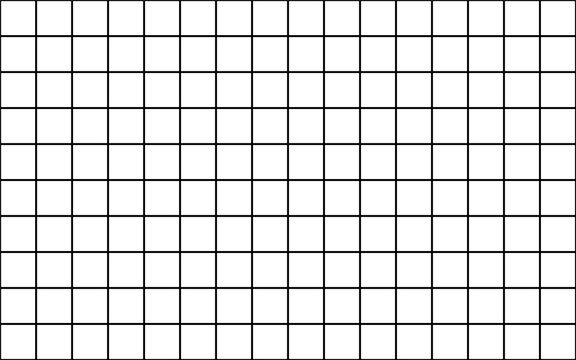
\includegraphics[scale=1.5]{figures/introduction/rect_grid.jpg}}
    }
    \caption{Plane decomposition into rectangular grid}
    
\end{figure}

Building ahead of these ideas and problems I will present a novel image compression codec \textbf{FRIF} (\textbf{FR}actal \textbf{I}mage \textbf{F}ormat)
which presents a new idea of fractal lattice decomposition of an image with discrete wavelet transform applied to each fractal region. Such grid
has a certain amount of interesting properties that could be leveraged in mentioned image compression methods:
\begin{itemize}
    \item Complex numeral systems fractals have a highly irregular boundary
    \item Since each fractal has 6 immediate neighbors, we get an hexagonal grid which allow inferring contexts and 
        predictions from a larger set
    \item Self-similarity relation of each fractal can benefit from wavelet transform decomposition
\end{itemize}
\begin{figure}[ht]
    \centering
    {
        \setlength{\fboxsep}{0pt}
        \setlength{\fboxrule}{1pt}
        \fbox{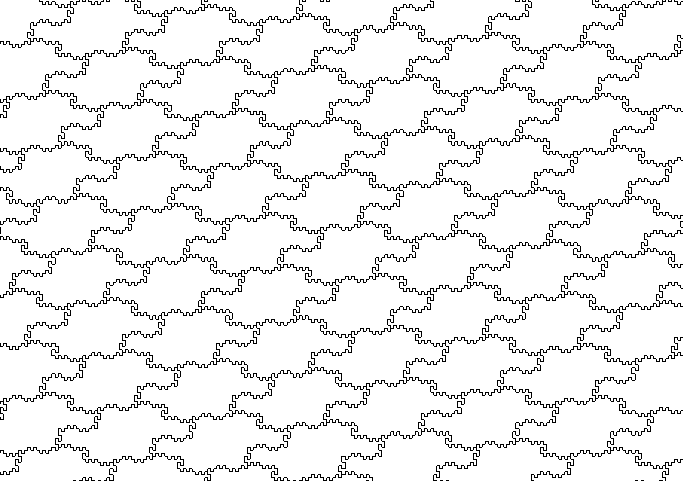
\includegraphics[scale=1.5]{figures/introduction/fractal_grid.png}}
    }
    \caption{Plane decomposition into tame-twindragon fractals}

\end{figure}
Along with the thesis implementation of the codec will be presented with comparisons to the existing lossless and lossy
popular approaches.
Experiments will be carried out over 3 datasets: kodak \cite{kodakdataset}, CID22 \cite{CID22} and JSI31 \cite{J31}
to collect average bits per pixel value corresponding to the compression ratio and SSIM2 metric to assess image quality after quantization.

Aim of this thesis is not to beat current sophisticated compression models with FRIF, but 
to measure performance of a quite different approach. The remainder of this thesis is organized as follows:
Section 2 presents the preliminaries required to state the compression algorithm, including complex-based numeral systems, wavelet transform and chosen entropy encoder.
Section 3 fully describes the FRIF compression algorithm, including all stages of compression and chosen image format to store compressed images on disk, giving the official
and full specification of this compression scheme. 
Section 4 showcases experiments taken to measure performance of codec, including metrics like bits per pixel or the quality of compressed image on lossy compression. 
Finally, section 5 reviews the codec and states the conclusion of this novel and unique approach.












